% !TEX TS-program = pdflatex
% !TEX encoding = UTF-8 Unicode

% This is a simple template for a LaTeX document using the "article" class.
% See "book", "report", "letter" for other types of document.

\documentclass[11pt]{article} % use larger type; default would be 10pt

\usepackage[utf8]{inputenc} % set input encoding (not needed with XeLaTeX)

%%% Examples of Article customizations
% These packages are optional, depending whether you want the features they provide.
% See the LaTeX Companion or other references for full information.

%%% PAGE DIMENSIONS
\usepackage{geometry} % to change the page dimensions
\geometry{a4paper} % or letterpaper (US) or a5paper or....
% \geometry{margin=2in} % for example, change the margins to 2 inches all round
% \geometry{landscape} % set up the page for landscape
%   read geometry.pdf for detailed page layout information

\usepackage{graphicx} % support the \includegraphics command and options
\usepackage{listings}
% \usepackage[parfill]{parskip} % Activate to begin paragraphs with an empty line rather than an indent

%%% PACKAGES
\usepackage{booktabs} % for much better looking tables
\usepackage{array} % for better arrays (eg matrices) in maths
\usepackage{paralist} % very flexible & customisable lists (eg. enumerate/itemize, etc.)
\usepackage{verbatim} % adds environment for commenting out blocks of text & for better verbatim
\usepackage{subfig} % make it possible to include more than one captioned figure/table in a single float
% These packages are all incorporated in the memoir class to one degree or another...

%%% HEADERS & FOOTERS
\usepackage{fancyhdr} % This should be set AFTER setting up the page geometry
\pagestyle{fancy} % options: empty , plain , fancy
\renewcommand{\headrulewidth}{0pt} % customise the layout...
\lhead{}\chead{}\rhead{}
\lfoot{}\cfoot{\thepage}\rfoot{}

%%% SECTION TITLE APPEARANCE
\usepackage{sectsty}
\allsectionsfont{\sffamily\mdseries\upshape} % (See the fntguide.pdf for font help)
% (This matches ConTeXt defaults)

%%% ToC (table of contents) APPEARANCE
\usepackage[nottoc,notlof,notlot]{tocbibind} % Put the bibliography in the ToC
\usepackage[titles,subfigure]{tocloft} % Alter the style of the Table of Contents
\renewcommand{\cftsecfont}{\rmfamily\mdseries\upshape}
\renewcommand{\cftsecpagefont}{\rmfamily\mdseries\upshape} % No bold!

%%% END Article customizations

%%% The "real" document content comes below...
\author{Li Jing}

\title{Partly BEC image fitting}

\begin{document}
\maketitle
\section{Density Distribution}
In theory, partly BEC has following density distribution:
\begin{equation}
n(\textbf{r}) = n_{th}Li_{3/2}(\prod_{i=1}^3\exp(-x_i^2/x_{i,th,0}^2)) + n_c\max(1-\sum_{i=1}^3\frac{x^2}{x_{i,c,0}^2}, 0)
\end{equation}
where $n_th$ is thermal atom number, $n_c$ condensated atom number. 
$Li$ is polylog function, whose definition is 
\begin{equation}
Li_{n}(z) = \sum_{k=1}^{\infty}\frac{z^k}{k^n}
\end{equation}

However, polylog function is quite difficult to use.
\begin{enumerate}
\item In matlab, polylog can only work for integal $n$.
\item In python, there is polylog in package \textbf{mpmath}. But it is in type \textbf{mpc}.
\item In order to fit, this function should work for array.
\end{enumerate}

So usually, we replace polylog by Gaussian, which is good enough for thermal clouds.

NOTE: for fermion fitting, we should not replace polylog by Gaussian. Because the most important property in fermion $T/T_F$ just represents the difference between polylog and Gaussian.

Now we can write down the approximate density distribution of the atom clouds.
\begin{equation}
n(\textbf{r}) = n_{th}\exp(-\sum_{i=1}^3x_i^2/x_{i,th,0}^2) + n_c\max(1-\sum_{i=1}^3\frac{x^2}{x_{i,c,0}^2}, 0)
\end{equation}


\section{fitting function}
Our images are 2D. So we need to integrat our funciton in one dimension.
\begin{equation}
n_{2D} = n_{th}\exp(-\sum_{i=1}^2x_i^2/x_{i,th,0}^2) + n_c\max(1-\sum_{i=1}^2\frac{x^2}{x_{i,c,0}^2}, 0)^{\frac{3}{2}}
\end{equation}

But 2D image is still quite difficult to fit, or very slow.
So usually, we integrate the image to 1D and fit these two directions separately.
That is, we slide the image in x axis to fit y-distribution and then repeat by change x and y.
Then, we need our 1D distribution:
\begin{equation}
n_{1D} = n_{th}\exp(-x_i^2/x_{i,th,0}^2) + n_c\max(1-\frac{x^2}{x_{i,c,0}^2}, 0)^{2}
\end{equation}

\section{Pseudo Code for fitting}
% \begin{listing}
\begin{lstlisting}
function 2D_partlyBEC_fit(2D_image):
	\\ get 1D slides
	slidesX = sum(2D_image, 0);
	slidesY = sum(1D_image, 1);
	\\ define 1D distribution inside 2D fit:
	\\ CENTER is position for cloud center
	\\ SIGMA is guassian size, WIDTH is parabolic size, 
	\\ OFFSET is background value. 
	\\ N_G and N_P are atom numbers respectively. 
	\\ x is coordinate.
	function 1D_partlyBEC(x, CENTER, SIGMA, WIDTH, N_G, N_P, OFFSET):
		return OFFSET + N_G * (-(x-CENTER)^2/SIGMA^2)
			+ N_P * max(0, 1-(x-CENTER)^2/WIDTH^2)
	\\ then do initial guess. This step is very important.
	Do initial guess

	\\ use built-in fit functions
	[centerX, sigmaX, widthX, n_GX, n_PX, offsetX] 
	= built-in-fit-function(1D_partlyBEC, slidesX, initial guess)

	[centerY, sigmaY, widthY, n_GY, n_PY, offsetY] 
	= built-in-fit-function(1D_partlyBEC, slidesY, initial guess)
	\\ combine two directions
	Transfer results to 2D

	return output
\end{lstlisting}

NOTE: 
{\begin{itemize}
\item Initial guess is very important before fit.
\item Validations that make sure atom number positive are useful.
\item Transfers from 1D to 2D are required before output.
\item In python, $curve\_fit$ in scipy is good for fit.
\end{itemize}



\section{Example}
\begin{figure}[htbp]
	\centering
	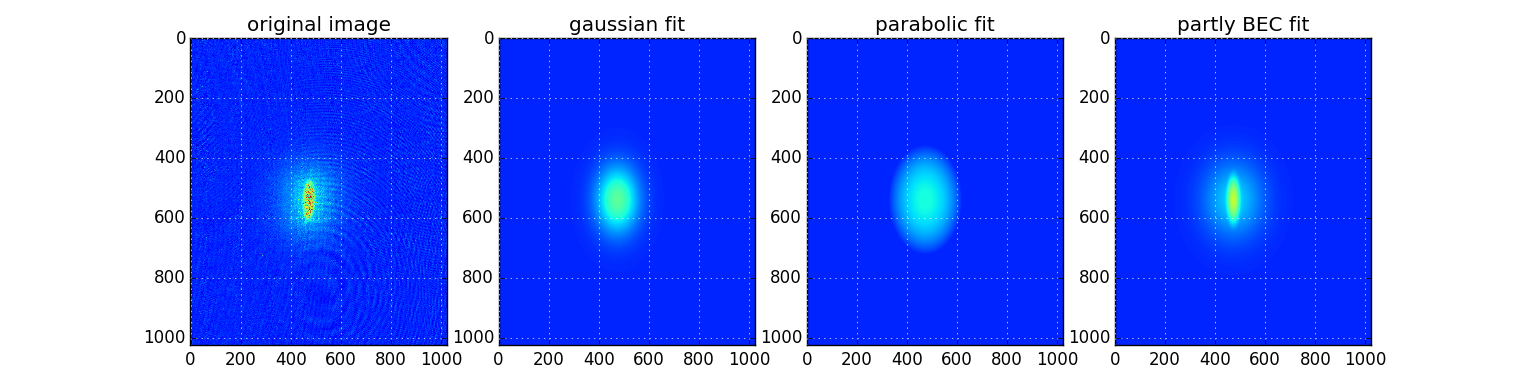
\includegraphics[width=1\textwidth]{1.png}
	\caption{60\% condensate}
	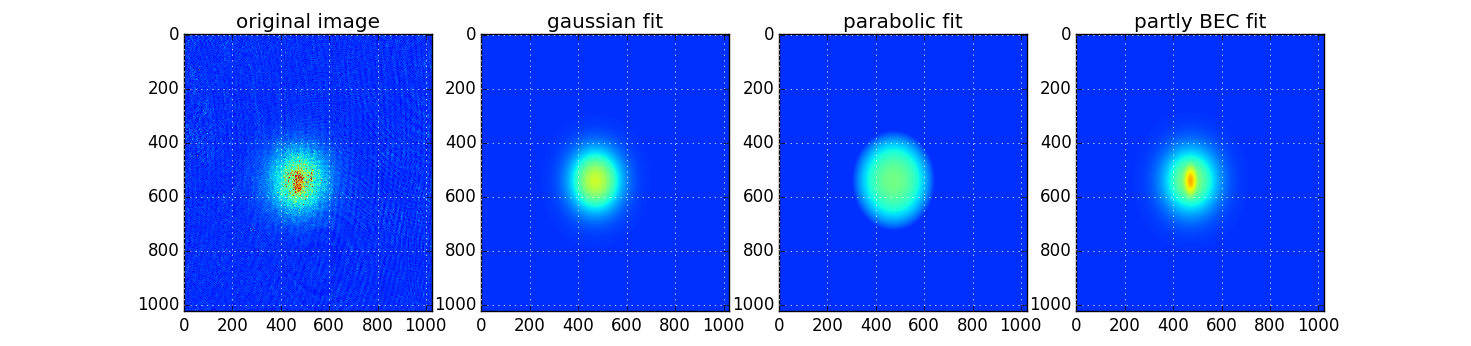
\includegraphics[width=1\textwidth]{2.png}
	\caption{30\% condensate}
\end{figure}



\end{document}

